% Niveau :      PCSI *
% Discipline :  Géné
% Mots clés :   Diagrammes E-pH

\begin{exercise}{Hydrométallurgie du zinc}{2}{PCSI}
{Chimie générale, Réactions acidobasiques, Oxydoréduction, Diagrammes E-pH}{bermu}

Cet exercice décrit schématiquement le processus d'extraction chimique du zinc à partir de la calcine, un minerai contenant les oxydes mixtes de cuivre (CuO, Cu$_2$O), de zinc (ZnO) et d'autres métaux. 
On se limitera par la suite à ces deux métaux.

\begin{questions}
\questioncours Lecture et construction de diagrammes $E$-pH.
\vspace{-1em}\begin{EnvUplevel}
Dans la figure \ref{fig:EpHCu} en annexe est tracé le diagramme $E$-pH du zinc pour les espèces $\mathrm{Zn_{(s)}}$, $\mathrm{{Zn^{2+}}_{(aq)}}$, $\mathrm{{Zn(OH)_2}_{(s)}}$ et $\mathrm{ {[Zn(OH)_4]^{2-}}_{(aq)}}$. \\[1ex]
\textsl{On tracera les diagrammes avec des couleurs différentes sur la figure en annexe. \\
Il ne sera exigé de calculer que les pentes de chaque frontière (tracé rapide).}
\end{EnvUplevel}
\begin{parts}
    \part En justifiant, ajouter au diagramme les domaines de prédominance / d'existence de ces espèces.
    \part Quel est le potentiel standard du couple $\mathrm{{Zn^{2+}}_{(aq)} / {Zn}_{(s)}}$ ?
    \part Tracer le diagramme $E$-pH de l'eau en donnant les équations des différentes frontières. \\
    \`A quoi correspondent ces trois domaines d'un point de vue chimique (mis à part les domaines de prédominance de chaque espèce) ?
    \part \`A l'aide des données, tracer le diagramme $E$-pH du cuivre. \\
    On pourra tout d'abord tracer en pointillés le diagramme pour les espèces de n.o. 0 et +I, puis +I et +II séparément.
\end{parts}

\begin{EnvUplevel}
    On s'intéresse maintenant au traitement de la calcine.
    
    Tout d'abord, elle est dissoute par lixiviation acide par action à chaud de l'acide sulfurique concentré.
    
    Ensuite, on introduit du zinc solide en poudre dans la solution pour éliminer les impuretés (le cuivre nottament).
    
    Enfin, les ions zinc (II) sont réduits en zinc solide par dépot sur une électrode en zinc.
\end{EnvUplevel}
    \question \'Ecrire l'équation de réaction correspondant à la lixiviation acide pour le zinc (II).
    
    \question Peut-on augmenter le pH pour précipiter et éliminer les ions cuivres de la solution ?
    
    \question Justifier donc la stratégie retenue pour éliminer le cuivre en écrivant l’équation de la réaction correspondante.
    
    \question Comment élimine-t-on ces sous-produits ?
    
    \question Expliciter la dernière étape et écrire l'équation correspondante. Proposer un matériau pour la seconde électrode.
    
    \question Pourquoi n’est-il pas possible de réaliser cette étape avec les ions cuivre et fer encore en solution ?

\end{questions}

\paragraph{Données :}

\begin{itemize}
    \item différentes espèces du cuivre dans les CNTP :

\hspace{-2em}\begin{minipage}{.68\linewidth}
Potentiels standards $E^\circ$ : \\[1em]
\begin{tabularx}{0.99\linewidth}{rCCC}
    \hline
    & $\mathrm{{Cu^{2+}}_{(aq)} \,/\, {Cu^+}_{(aq)}}$
    & $\mathrm{{Cu^{2+}}_{(aq)} \,/\, {Cu}_{(s)}}$
    & $\mathrm{{O_2}_{(g)} \,/\, {H_2O}_{(\ell)}}$ \\
    $E^\circ$ (V) & 0,16 & 0,34 & 1,23 \\
    $E^\circ / \varepsilon^\circ$ & 3 & 6 & 21 \\ \hline\hline 
\end{tabularx}
\end{minipage}
\begin{minipage}{.32\linewidth}
Produits de solubilité p$K_s$ :

\begin{tabularx}{.99\linewidth}{rCC}
    \hline
    & $\mathrm{{Cu(OH)}_{(s)}}$
    & $\mathrm{{Cu(OH)_2}_{(s)}}$ \\
    p$K_s$  & 15 & 20 \\ \hline\hline 
\end{tabularx}
\end{minipage}

    \item on note $\varepsilon^\circ = \dfrac{RT}{\scr{F}} \ln10 = 59$ mV.

    \item les oxydes métalliques et les hydroxydes métalliques seront considérés comme équivalents :
    $$\text{En milieu aqueux : } \quad \mathrm{{M_x(OH)_{2y}}_{(s)} \quad \longleftrightarrow \quad \text{En milieu sec : } {M_xO_y}_{(s)}}$$
\end{itemize}


\end{exercise}

\begin{nopagebreak}
    \exerciselabelformat{Annexe Exercice \arabic{exercise} \quad --- \quad} \textsl{\`A rendre avec la copie.}
    
    \begin{figure}[H]
        \centering
        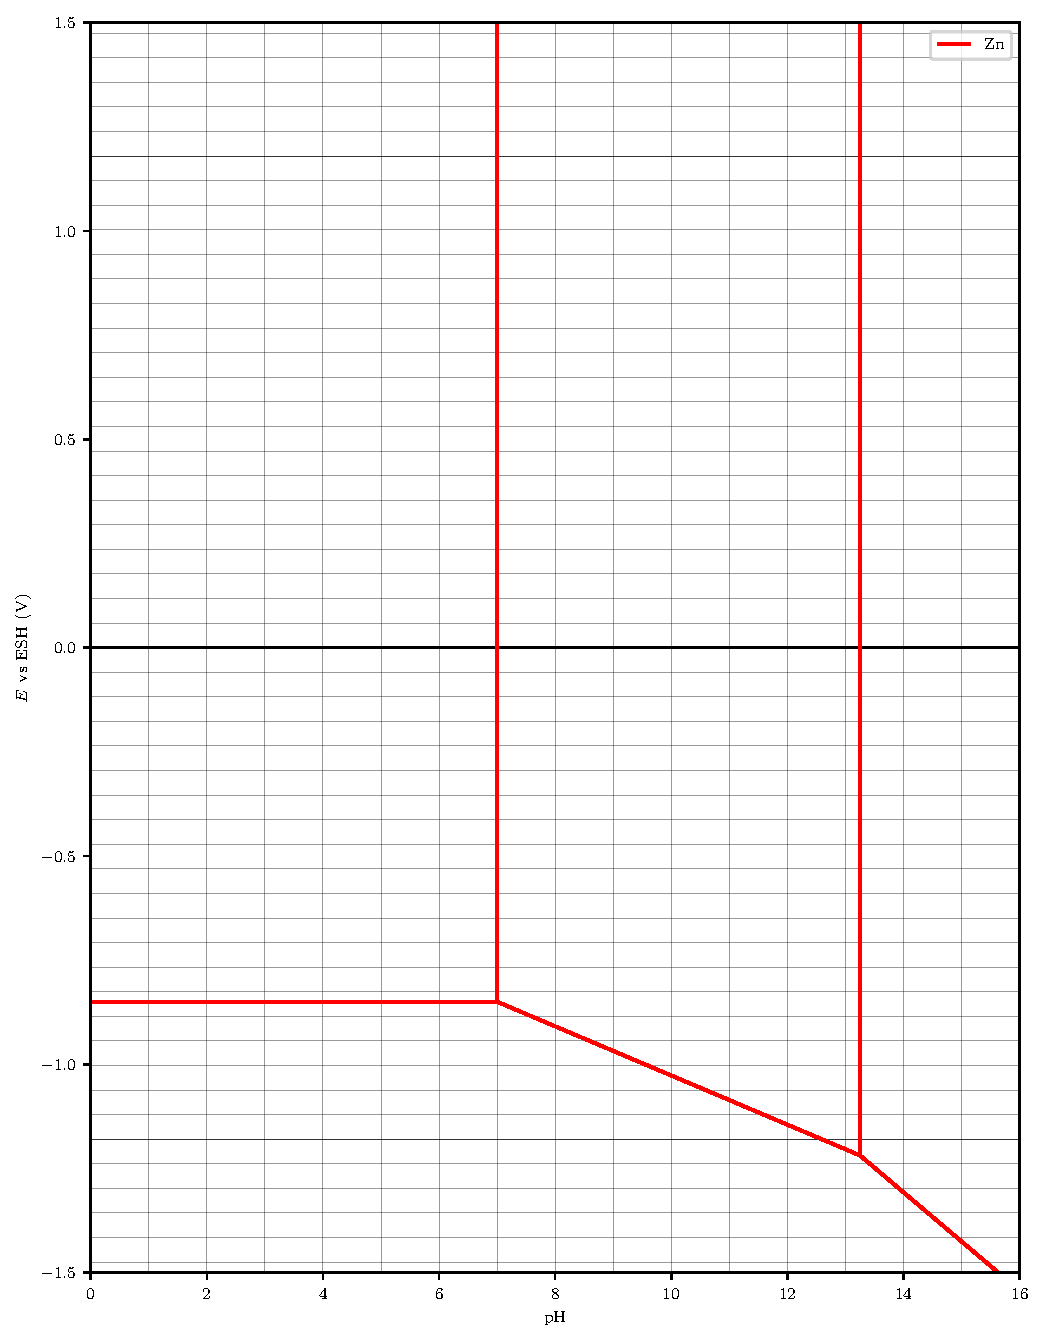
\includegraphics[width = \linewidth]{chimiePC/gene/E-pH-Zn.pdf}
        \caption{Diagramme $E$-pH du zinc avec une concentration de tracé de $10^{-2}$ M. \protect\linebreak
        Le quadrillage est de $\varepsilon^\circ = 59$ mV par 1 unité de pH.}
        \label{fig:EpHCu}
    \end{figure}
    
    \paragraph{Convention de tracé :}
\begin{itemize}
    \item les espèces en solution ont pour activité $c_\text{tr}/c^\circ = 10^{-2}$,
    \item les espèces gazeuses ont pour activité $p_\text{tr}/p^\circ = 10^{-2}$,
    \item les espèces solides ont pour activité $1$.
\end{itemize}

\end{nopagebreak}


\begin{solution}
\begin{questions}

\questioncours cf. le diagramme complété
\begin{parts}
    \part cf. cours pour la méthode.
    \part La demi-équation rédox couple $\mathrm{{Zn^{2+}}_{(aq)} / {Zn}_{(s)}}$ donne avec la relation de Nernst à la frontière $E = E^\circ + e^\circ/2 \log c_\text{tr}$, d'où $E^\circ = 0,79$ V.
    \part Le domaine central désigne le domaine de stabilité rédox de l'eau.
    \part \underline{n.o. 0 et +I :} on a  Cu$^+$ et Cu(OH) \emph{vs} Cu.
    \begin{itemize}
        \item Cu$^+$ / Cu : $E = 2 E^\circ\qty\Big(\mathrm{Cu^{2+} / Cu}) - E^\circ\qty\Big(\mathrm{Cu^{2+} / Cu^{+}}) + e^\circ \log c_\text{tr} \simeq 7 e^\circ$ ;
        \item Cu$^+$ / Cu(OH) : $\text{p}K_s = -\log c_\text{tr} + \text{p}K_e - pH$ d'où $\text{pH} = 1$ ;
        \item Cu(OH) / Cu : $\mathrm{Cu(OH) + H^+ + e^- = Cu + H_2O}$ donc pente de -0.06 V/u.pH.
    \end{itemize}
    
    \underline{n.o. +I et +II :} on a  Cu$^{2+}$ et Cu(OH)$_2$ \emph{vs} Cu$^+$ et Cu(OH).
    \begin{itemize}
        \item Cu$^{2+} / Cu^+$ : $E = E^\circ\qty\Big(\mathrm{Cu^{2+} / Cu^+}) + e^\circ \log c_\text{tr} \simeq 3 e^\circ$ ;
        \item Cu$^+$ / Cu(OH) : idem ;
        \item Cu$^{2+}$ / Cu(OH)$_2$ : $\text{p}K_s = -\log c_\text{tr} + \text{p}K_e - pH$ d'où $\text{pH} = 5$ ;
        \item Cu$^{2+}$ / Cu(OH) : $\mathrm{Cu^{2+} + H_2O + e^- = Cu(OH) + H^+}$ donc pente de +0.06 V/u.pH ;
        \item Cu(OH)$_2$ / Cu(OH) : $\mathrm{Cu(OH)_2 + H^+ + e^- = Cu(OH) + H_2O}$ donc pente de -0.06 V/u.pH.
    \end{itemize}
        
    Après tracé (en pointillés), on voit que Cu$^+$ dismute, et donc on a une frontière directe Cu$^{2+}$ / Cu à $E \simeq 5 e^\circ$.
\end{parts}

    \question $\mathrm{ZnO + 2 H^+ = Zn^{2+} + H_2O}$
    
    \question Si on augmente le pH, on va précipiter indistinctement les hydroxydes métalliques, donc ça ne marche pas.
    
    \question On voit sur le diagramme que Cu$^{2+}$ et Zn ne peuvent pas coexister. Ils vont donc réagir $$\mathrm{Cu^{2+} + Zn_{(s)} = Zn^{2+} + Cu_{(s)}}.$$
    
    \question Il suffit ensuite de filter le cuivre solide et le tour est joué.
    
    \question Il s'agit de réduire le zinc à la cathode : $\mathrm{Zn^{2+} + 2 e^- = Zn_{(s)}}$. Pour que la cathode soit l'électrode de zinc, il faut donc une anode avec un potentiel standard plus élevé comme le platine par exemple qui contrebalance avec une oxydation de l'eau
    $\mathrm{2 H_2O = O_2 + 4 H^+ + 4 e^-}$. De plus, le platine résiste au O$_2$ produit.

    \question Comme ils ont des potentiels standards plus élevés, ils réagiraient mieux et la méthode ne serait plus sélective.

\end{questions}

    \exerciselabelformat{Solution Annexe Exercice \arabic{exercise}.}
    
    \begin{figure}[H]
        \centering
        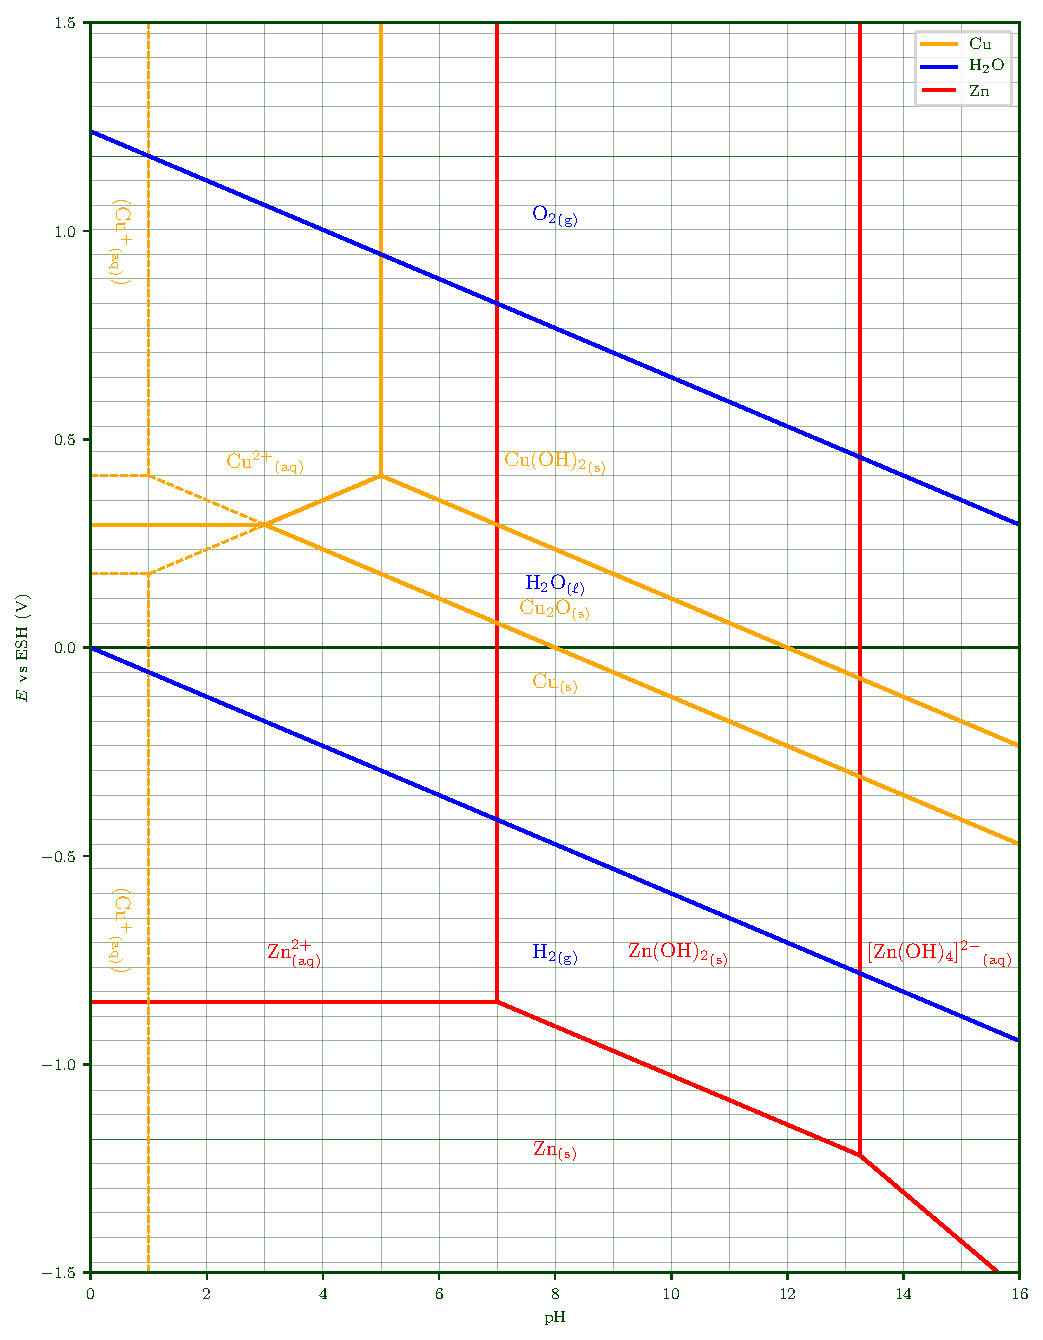
\includegraphics[width = \linewidth]{chimiePC/gene/E-pH-Zn-sol.pdf}
        \caption{Diagrammes $E$-pH superposés du cuivre, du zinc et de l'eau. \protect\linebreak
        Le quadrillage est de $\varepsilon^\circ = 59$ mV par 1 unité de pH.}
        \label{fig:EpHS-sol}
    \end{figure}

\end{solution}